\documentclass[10pt]{beamer}
 
\usepackage[utf8]{inputenc}
\usepackage{xcolor}
\usepackage{kotex}
\usepackage{enumerate}
\usepackage{mathtools}
\usepackage{multicol}
\usepackage{bbm}
\usepackage{subfig}
\usepackage{graphicx}
\usepackage{amsmath}
\usepackage{bbm}
\usepackage[algoruled, boxed, slide, noline]{algorithm2e}
\usepackage{booktabs}
\DeclareGraphicsExtensions{.pdf,.png,.jpg}
\usetheme[]{Madrid}

 
%Information to be included in the title page:
\title[Polynomial Acclerated Gibbs Sampling] 
{Polynomial Accelerated Gibbs Sampling}
 
\author[김동욱, 김민지, 김민우] 
{Dongwuk Kim, Minji Kim and Minwoo Kim}
\institute[SNU]{Seoul National University}
\date[\today]{\today}
 
\begin{document}

\begin{frame}
  \titlepage
\end{frame}

\AtBeginSection[]
{
  \begin{frame}
    \frametitle{Table of Contents}
    \tableofcontents[currentsection, hideothersubsections]
  \end{frame}
}
 
\section{1. Introduction}
\begin{frame}{Introduction}
    \begin{itemize}
        \item \emph{Our problem} is \emph{\color{blue}sampling from normal distirubions.}
        \item Gibbs sampler is commonly used because of simple implementaion 
        \item However, the Gibbs sampler is not efficient for a massive models.
        \item C. Fox and A.Parker(2017) proposed a generalized and accelerated Gibbs samplers which is fast for high-dimensional normal distributions.
        \item In this presentation, we review the paper of C. Fox and A. Parker(2017)
        - \emph{\color{blue}“Accelerated Gibbs sampling of normal distributions using matrix 
        splittings and polynomials”} -  Bernoulli 23.4B
        and show the reseult of the proposed algorithm re-written by \textit{Julia}.
    \end{itemize}
\end{frame}


\section{2. Problem setting and previous works}

\begin{frame}{Problem}
\begin{enumerate}
    \item We want to compute a sample
       $$
       \mathbf{y} \sim \mathbf{N}(0, A^{-1})
       $$
       , where $A$ is a given precision matrix. 
    \item An iterative samplers, such as \emph{\color{blue}Gibbs}, are good option when the dimension is high becuase of it's inexpensive cost per itertion and small computer memroy requirements. 
    \item If the precision matrix $A$ is sparse with $\mathcal{O}(n)$ non-zero elements, iterative methods cost only about $2n$ flops per iteration.
    \item So, our goal is find an Iterative method which converges in small iterations, for example, significantly less than $\mathcal{O}(n^2)$ iterations.
\end{enumerate}
\end{frame}

\begin{frame}{Gibbs Sampling from a normal distribution}
    \begin{algorithm}[H]
        \KwIn{Precision matrix $\mathbf{A}$, initial state $\mathbf{y}^{(0)} = 
        (y_1^{(0)}, y_2^{(0)}, \dots, y_n^{(0)})^T$}, and maximum iteration $k_{\max}$ \\
        \KwOut{$\mathbf{y}^{(0)},\mathbf{y}^{(1)},\mathbf{y}^{(2)} 
        \dots, \mathbf{y}^{(k_{\max})}$, 
        where $\mathbf{y}^{(k)} \overset{\mathcal{D}}{\longrightarrow} \mathbf{N}(0, \mathbf{A}^{-1})$}
        \For{$k = 1, 2, \dots, k_{\max}$}{
            \For{$i = 1, 2, \dots, n$}{
            sample $z \sim \mathbf{N}(0, 1)$; \newline
            $y_i^{(k)} = \frac{z}{\sqrt{a_{ii}}} - \frac{1}{a_{ii}}
            (\sum_{j>i} a_{ij}y_j^{(k-1)} - \sum_{j<i}a_{ij}y_j^{(k)})$
            }
        }
        \caption{Component-sweep Gibbs sampling using a precision matrix $\mathbf{A}$}
    \end{algorithm}

    The iteration can be written in the matrix form,
    \begin{equation}
        \mathbf{y}^{(k+1)} = -\mathbf{D}^{-1}\mathbf{L}\mathbf{y}^{(k+1)} - \mathbf{D}^{-1}\mathbf{L}^T\mathbf{y}^{(k)} + \mathbf{D}^{-1/2}\mathbf{z}^{(k)}
    \end{equation}
    , where $\mathbf{z}^{(k)} \sim N(0, \mathbf{I})$, $\mathbf{D} = \text{diag}(\mathbf{A})$, and 
    $\mathbf{L}$ is the strictly lower triangluar part.
\end{frame}

\begin{frame}{Splitting iterative linear solvers}
The iterative method for solving $\mathbf{A}\mathbf{x}=\mathbf{b}$ split the matrix 
$\mathbf{A} = \mathbf{M} - \mathbf{N}$, where $\mathbf{M}$ is invertible and easy to invert.
Then $\mathbf{A}\mathbf{x} = \mathbf{M}\mathbf{x} - \mathbf{N}\mathbf{x} = \mathbf{b}$ or
$$
    \mathbf{x} = \mathbf{M}^{-1}\mathbf{N}\mathbf{x} - \mathbf{M}^{-1}\mathbf{b}
$$
Thus a solution to $\mathbf{A}\mathbf{x}=\mathbf{b}$ is a fixed point of iteration
    \begin{equation}
        \mathbf{x}^{(k+1)} = \mathbf{M}^{-1}\mathbf{N}\mathbf{x}^{(k)} - \mathbf{M}^{-1}\mathbf{b}.
    \end{equation}
The iterative solution is convergent(i.e., $\mathbf{x}^{(k)} \rightarrow \mathbf{A}^{-1}\mathbf{b}$)
if and only if 
$$\mathcal{\rho}(\mathbf{M}^{-1}\mathbf{N}) < 1$$ 
,where $\mathcal{\rho}(\cdot)$ is the spectral radius of a matrix. 
Let the error at step $k$ be $\mathbf{e}^{(k+1)} =\mathbf{x}^{(k+1)} - \mathbf{A}^{-1}\mathbf{b}.$
Then it's well known(e.g. \emph{Axelsson}[1]) that
    \begin{equation}
        \lim_{k \to \infty}
        \bigg(\frac{\|\mathbf{e}^{(k+1)}\|_2}{\|\mathbf{e}^{(0)}\|_2}\bigg)^{1/k}  
        = \mathcal{\rho}(\mathbf{M}^{-1}\mathbf{N})
    \end{equation}
\end{frame}

\begin{frame}{Splitting iterative linear solvers}
For a symmetric matrix $\mathbf{A}$, let $\mathbf{A} = \mathbf{L} + \mathbf{D} + \mathbf{L}^T$
, where $\mathbf{L}$ is a strictly lower triangular part and $\mathbf{D}$ is a diagonal part.
\begin{table}[]
    \begin{tabular}{@{}lll@{}}
    \toprule
     Splitting &  $\mathbf{M}$ &  Convergence\\ \midrule
     Richardson & $\frac{1}{\omega}\mathbf{I}$  & $0 < \omega < \frac{2}{\rho(\mathbf{A})}$ \\
     Jacobi &  $\mathbf{D}$ & $\mathbf{A}$ strictly diagonally dominant \\
     Gauss-Seidel(GS) & $\mathbf{D} + \mathbf{L}$ & always \\
     SOR & $\frac{1}{\omega}\mathbf{D} + \mathbf{L}$ & $0 < \omega < 2$ \\
     SSOR & $\frac{\omega}{2 - \omega}\mathbf{M}_{\text{SOR}}\mathbf{D}^{-1}\mathbf{M}_{\text{SOR}}^T$ 
     & $0 < \omega < 2$ \\ \bottomrule
    \end{tabular}
\end{table}
For the \emph{\color{blue}Gauss-Seidel} method, (2) becomes
    \begin{equation}
        \mathbf{x}^{(k+1)} = -\mathbf{D}^{-1}\mathbf{L}\mathbf{x}^{(k+1)} - \mathbf{D}^{-1}\mathbf{L}^T\mathbf{x}^{(k)} + \mathbf{D}^{-1}\mathbf{b}.
    \end{equation}
Note that the gibbs sampler iteration (1) and linear solver's (4) are almost same. 
\end{frame}

\begin{frame}{Equivalence of linear solvers and Gibbs samplers}
    \begin{theorem}[Equivalence of iterative linear solvers and Gibbs samplers] % Thm 1
        Let $\mathbf{A} = \mathbf{M} - \mathbf{N}$ be a splitting with $\mathbf{M}$ invertible, and let
        $\pi(\cdot)$ be some fixed probability distribution with zero mean and fixed non-zero covariance.
        For any fixed vector $\mathbf{b}$, and random vectors 
        $\mathbf{c}^{(k)} \overset{\text{i.i.d.}}{\sim} \pi$, $k = 0, 1, 2, \dots,$ 
        the stationary linear iteration
        \begin{equation}
            \mathbf{x}^{(k+1)} = \mathbf{M}^{-1}\mathbf{N}\mathbf{x}^{(k)} + \mathbf{M}^{-1}\mathbf{b}
        \end{equation}
        converges, with $\mathbf{x}^{(k)} \to \mathbf{A}^{-1}\mathbf{b}$ as $k \to \infty$ whatever
        the initial vector $\mathbf{x}^{(0)}$, if and only if there exists a distribution $\Pi$ such that
        the stochastic iteration
       \begin{equation}
            \mathbf{y}^{(k+1)} = \mathbf{M}^{-1}\mathbf{N}\mathbf{y}^{(k)} + \mathbf{M}^{-1}\mathbf{c}^{(k)}
        \end{equation}
        converges in distribution on $\Pi$, with $\mathbf{y}^{(k)} \overset{\mathcal{D}}{\to} \Pi$ as
        $k \to \infty$ whatever the initial state $\mathbf{y}^{(0)}$.
    \end{theorem}
\end{frame}

\begin{frame}{Sampling from normal distributions using matrix splittings}
    \begin{theorem}[Convergence of first and second moments] % Thm 2
        Let $\mathbf{A}$ be SPD, $\mathbf{A} = \mathbf{M} - \mathbf{N}$ be a convergent splitting,
        $\mathbf{\mu}$ a fixed vector, and $\pi(\cdot)$ a fixed probability distribution with finite mean
        $\mathbf{\nu}$ and non-zero covariance $\mathbf{V}$. Consider the stochastic iteration (6) where
        $\mathbf{c}^{(k)} \overset{\text{i.i.d.}}{\to}\pi$, $k = 0, 1, 2, \dots .$ Then, whatever the starting
        state $\mathbf{y}^{(0)}$, the following are equivalent:
        \begin{enumerate}
            \item $\textbf{E}[\mathbf{c}^{(k)}] = \mathbf{\nu}$ and 
            $\textbf{Var}(\mathbf{c}^{(k)}) = \mathbf{V} = \mathbf{M}^T + \mathbf{N}$;
            \item the iterates $\mathbf{y}^{(k)}$ converges in distribution to some distribution $\Pi$ that
            has mean $\mathbf{\mu} = \mathbf{A}^{-1}\mathbf{\nu}$ and covariance matrix $\mathbf{A}^{-1}$;
            in particular $\textbf{E}[\mathbf{y}^{(k)}] \to \mathbf{\mu}$ and 
            $\textbf{Var}(\mathbf{y}^{(k)}) \to \mathbf{A}^{-1}$ as $k \to \infty$.
        \end{enumerate}
    \end{theorem}
    \begin{itemize}
        \item This theorem shows \emph{\color{blue} how to design} the noise distribution $\pi$ 
        so that the limit distribution
        $\Pi$ has a desired mean $\mu$ and covariance $\Sigma = \mathbf{A}^{-1}$.
        \item If we set $\pi = \text{N}(\mathbf{\nu}, \mathbf{V})$ then the following are equivalent:
        (i) $\mathbf{V} = \mathbf{M}^T + \mathbf{N}$; 
        (ii) $\mathbf{y}^{(k)} \overset{\mathcal{D}}{\to} \mathbf{N}(\mathbf{\mu}, \mathbf{A}^{-1})$
        where $\mathbf{\mu} = \mathbf{A}^{-1}\mathbf{\nu}$.
    \end{itemize}
\end{frame}

\begin{frame}{Sampling from normal distributions using matrix splittings}
    \begin{algorithm}[H]
        \KwIn{SPD precision matrix $\mathbf{A} = \mathbf{M} - \mathbf{N}$ to be convergent splitting
        , initial state $\mathbf{y}^{(0)}$ and maximum iteration $k_{\max}$} 
        \KwOut{$\mathbf{y}^{(k)}$ approximately distributed as $\mathbf{N}(0, \mathbf{A}^{-1})$}
        \For{$k = 0, 1, \dots, k_{\max}$}{
            sample $z \sim \mathbf{N}(0, \mathbf{M}^T + \mathbf{N})$; \newline
            $\mathbf{y}^{(k+1)} = \mathbf{M}^{-1}(\mathbf{N}\mathbf{y}^{(k)} + \mathbf{c}^{(k)})$
        }
        \caption{Stationary sampler of  $\mathbf{N}(0, \mathbf{A}^{-1})$}
    \end{algorithm}
\end{frame}

\begin{frame}{Sampling from normal distributions using matrix splittings}
    \begin{algorithm}[H]
        \KwIn{The SOR splitting $\mathbf{M}, \mathbf{N}$ of $\mathbf{A}$, relaxation parameter $\omega$
        , initial state $\mathbf{y}$ and maximum iteration $k_{\max}$} 
        \KwOut{$\mathbf{y}$ approximately distributed as $\mathbf{N}(0, \mathbf{A}^{-1})$}
        
        set $\gamma = (\frac{2}{\omega} - 1)^{1/2}$; \newline
        
        \For{$k = 1, \dots, k_{\max}$}{
            sample $\mathbf{z} \sim \mathbf{N}(0, \mathbf{I})$; \newline
            $\mathbf{x} \leftarrow 
            \mathbf{M}^{-1}(\mathbf{N}\mathbf{y} + \gamma\mathbf{D}^{1/2}\mathbf{Z})$; \newline
            sample $\mathbf{z} \sim \mathbf{N}(0, \mathbf{I})$; \newline
            $\mathbf{y} \leftarrow 
            \mathbf{M}^{-T}(\mathbf{N}^T\mathbf{x} + \gamma\mathbf{D}^{1/2}\mathbf{Z})$
        }
        \caption{SSOR sampling from $\mathbf{N}(0, \mathbf{A}^{-1})$}
    \end{algorithm}
    
    \begin{itemize}
        \item This is how the \emph{\color{blue} IterativeSolvers.jl}, Julia package, implement
        the SSOR-iterative solver. The only things to change is
        $\gamma\mathbf{D}^{1/2}\mathbf{Z}$ to $\mathbf{b}$, where the problem is 
        $\mathbf{A}\mathbf{x} = \mathbf{b}$.
    \end{itemize}
\end{frame}


\section{3. Proposed method and Theory}
\begin{frame}{Accleration of linear solvers by polynomials}
For a set of \emph{\color{blue}acceleration parameters} $\{ \{\alpha_k\}, \{\tau_k\}\}$, 
let's introduce the second order iteration
    \begin{equation}
        \mathbf{x}^{(k+1)} = (1-\alpha_k)\mathbf{x}^{(k-1)} + \alpha_k \mathbf{x}^{(k)} +
        \alpha_k\tau_k\mathbf{M}^{-1}(\mathbf{b} - \mathbf{A}\mathbf{x}^{(k)}).
    \end{equation}
At the first step, $\alpha_0 = 1$ and 
$\mathbf{x}^{(1)} = \mathbf{x}^{(0)} + \tau_0\mathbf{M}^{-1}(\mathbf{b} - \mathbf{A}\mathbf{x}^{(0)})$.
Next, generate a (k+1)st order polynomial $P_{k+1}$ recursively as
    \begin{equation}
        P_{k+1}(\lambda) = (\alpha_k - \alpha_k\tau_k\lambda)P_k(\lambda) + (1-\alpha_k)P_{k-1}(\lambda).
    \end{equation}
Then the $k$-step error $\mathbf{e}^{(k)} = \mathbf{x}^{(k)} - \mathbf{A}^{-1}\mathbf{b}$ may be
written as 
    \begin{equation}
        \mathbf{e}^{(k+1)} = P_k(\mathbf{M}^{-1}\mathbf{A}) \mathbf{e}^{(0)}    
    \end{equation}
, which can be compared directly to (5).
\end{frame}

\begin{frame}{Accleration of linear solvers by polynomials}
When estimates of the extreme eigenvalues $\lambda_{\min}$, $\lambda_{\max}$ of 
$\mathbf{M}^{-1}\mathbf{A}$ are available($\lambda_{\min}$, $\lambda_{\max}$ are real when
$\mathbf{M}, \mathbf{N}$ are symmetric), then following coefficients
$\{ \{\alpha_k\}, \{\tau_k\}\}$ generate the \emph{\color{blue}scaled Chebyshev} polynomials

\begin{equation}
    \tau_k = \frac{2}{\lambda_{\max} + \lambda_{\min}}, \quad
    \beta_k = \bigg( \frac{1}{\tau_k} - \beta_{k-1}
    \bigg( \frac{\lambda_{\max} - \lambda_{\min}}{4}
    \bigg)^2 \bigg)^{-1}, \quad
    \alpha_k = \frac{\beta_k}{\tau_k}
\end{equation}
, where $\alpha_0 = 1$ and $\beta_0 = \tau_0$.
\begin{itemize}
    \item We denote the $k$-th oreder Chebyshev polynomial as $\mathcal{Q}_k$.
    \item Note that these parameters are independent of the iterates $\{\mathbf{x}^{(k)}\}$.
    \item $\mathbf{M}$ is required to be symmetric, applying Chebyshev acceleration to SSOR
    is a common paring.
\end{itemize}
\end{frame}

\begin{frame}{Acceleration of linear solvers by polynomials}
From \emph{Axelsson},
\begin{equation}
    \mathcal{Q}_k = \underset{{P_k \in \mathbb{P}_k}}{\text{argmin}}
    \bigg(
    \underset{\lambda \in [\lambda_{\min}, \lambda_{\max}]}{\max} |P_k(\lambda)|
    \bigg),
\end{equation}
where $\mathbb{P}_k$ is a space of $k$th order polynomials. The optimal value is
\begin{equation}
    \underset{\lambda \in [\lambda_{\min}, \lambda_{\max}]}{\max} |\mathcal{Q}_k(\lambda)|
    = \frac{2\sigma^k}{1 + \sigma^{2k}}, \quad
    \text{where }
    \sigma = \frac{1 - \sqrt{\lambda_{\min}/\lambda_{\max}}}
    {1 + \sqrt{\lambda_{\min}/\lambda_{\max}}} \in [0, 1).
\end{equation}
From (9), 
$\mathbf{e}^{(k+1)} = \mathcal{Q}_k(\mathbf{M}^{-1}\mathbf{A})\mathbf{e}^{(0)}$ and
then the asymptotic convergence factor is bounded above by
\begin{equation}
    \lim_{k \to \infty} \{\max |\mathcal{Q}_k(\lambda)|\}^{1/k} = \sigma 
\end{equation}
\emph{Axelsson} also shows the convergence factor of non-accelerated iterative solver is
bounded below by $\rho = \frac{1 - \lambda_{\min}/\lambda_{\max}}
{1 + \lambda_{\min}/\lambda_{\max}}.$
Then $\sigma < \rho$ always holds, 
so the Chebyshev acceleration \emph{\color{blue}really accelerate} a calculation procedures.

\end{frame}

\begin{frame}{Acceleration of Gibbs sampling by polynomials}
    \begin{itemize}
        \item By slightly chainging (7), we can consider the second order stochastic iteration
            \begin{equation}
                \mathbf{y}^{(k+1)} = 
                (1-\alpha_k)\mathbf{y}^{(k-1)} + \alpha_k \mathbf{y}^{(k)} +
                \alpha_k\tau_k\mathbf{M}^{-1}(\mathbf{c}^{(k)} - \mathbf{A}\mathbf{y}^{(k)}).
            \end{equation}
            Only diffrenet thing is the vector $\mathbf{b}$ 
            has been replaced by a random vector $\mathbf{c}^{(k)}$.
        \item Next, introduce some coefficients $a_k, b_k, \kappa_k$ defined by
            $a_k = (2-\tau_k)/\tau_k + (b_k-1)(1/\tau_k + 1/\kappa_k - 1)$, 
            $b_k = 2\kappa_k(1-\alpha_k)/(\alpha_k \tau_k) + 1$, 
            $\kappa_{k+1} = \alpha_k \tau_k + (1-\alpha_k)\kappa_k$, and $\kappa_1 = \tau_0$.
        \item Also, suppose that $\{\{\alpha_k\}, \{\tau_k\}\}$ that are independent of 
            $\{\mathbf{x}^{(k)}\}$.
        \item Then (14) \emph{\color{blue}converges in distribution to our targe distribution} if the polynomial accerated linear solver converges.
    \end{itemize}
\end{frame}

\begin{frame}{Main Results}
    \begin{theorem}[Accelerated Gibbs sampler]
    Let $\mathbf{A}$ be SPD and $\mathbf{A} = \mathbf{M} - \mathbf{N}$ be a symmetric splitting. Define an noise vectors 
    $\mathbf{c}^{(k)} \overset{ind.}{\sim} (\mathbf{\nu}, a_k \mathbf{M} + b_k \mathbf{N})$.
        \begin{enumerate}
            \item If the accelerated linear solver (7) converges to $\mathbf{A}^{-1}\mathbf{b}$
                then the accelerated stochastic iteration (14)
                converges to a distribution with moments $(\mathbf{A}^{-1}\nu, \mathbf{A}^{-1}).$ 
                Furthermore, if the $\{\mathbf{c}^{(k)}\}$ are normal, then
                \begin{equation}
                    \mathbf{y}^{(k)} \overset{\mathcal{D}}{\to} 
                    \mathbf{N}(\mathbf{\mu} = \mathbf{A}^{-1}\nu, \mathbf{A}^{-1}).
                \end{equation}
            \item $\mathbf{E}(\mathbf{y}^{(k)})-\mathbf{A}^{-1}\nu 
            = P_k(\mathbf{M}^{-1}\mathbf{A})(\mathbf{E}(\mathbf{y}^{(0)})-\mathbf{A}^{-1}\nu)
            \to 0$
            \item $\mathbf{Var}(\mathbf{y}^{(k)})-\mathbf{A}^{-1} 
            = P_k(\mathbf{M}^{-1}\mathbf{A})(\mathbf{Var}(\mathbf{y}^{(0)})-\mathbf{A}^{-1})
            P_k(\mathbf{M}^{-1}\mathbf{A})^T \to 0$.
        \end{enumerate}
    \end{theorem}
    \begin{itemize}
        \item Chebyshev polynomial accelerated normal sampler is guaranteed to
        converge faster than any other acceleration scheme that has the parameters 
        $\{ \alpha_k, \tau_k \}$ independent of the iterates $\{\mathbf{y}^{(k)}\}$.
    \end{itemize}
\end{frame}

\section{4. Computed examples}

\begin{frame}{Example 1. 10 by 10 lattice sparse precision matrix}
We generate the $\mathbf{A}$ matrix in Sec 6.1 of [C. Fox and A. Parker] by Julia v1.2.0.
The following plot is sparsity pattern of $\mathbf{A}$.
\begin{figure}
    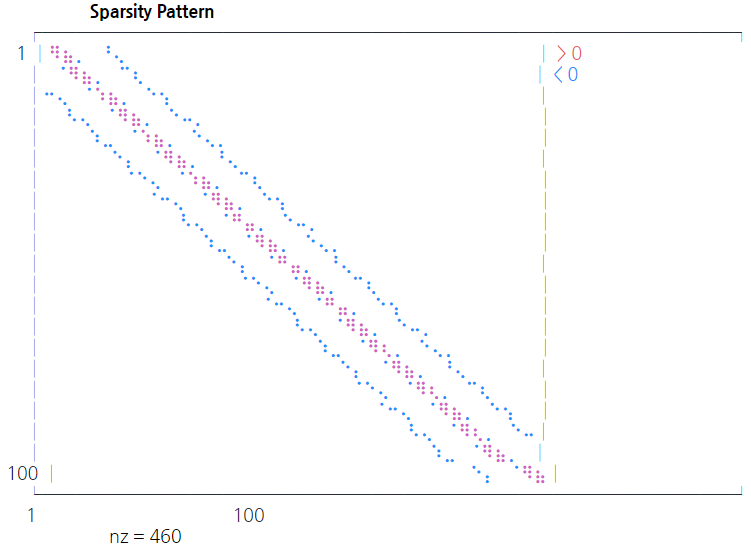
\includegraphics[width=0.6\columnwidth]{spy_A.png}
    \caption{Sparsity pattern of A}
    \label{fig:spyA}
\end{figure}
\end{frame}

\begin{frame}{Example 1. 10 by 10 lattice sparse precision matrix}
Following table is our calculation results for solving $Ax = b$. 
Note that there are small diffrences comparing to the paper's results
but there diffrences are negligible.
\begin{table}[]
    \begin{tabular}{@{}lllll@{}}
    \toprule
    Solver & $\omega$ & $\mathcal{\rho}(\mathbf{M}^{-1}\mathbf{N})$ & Number of iterations & Flops/Iteration \\ \midrule
    Richardson   & 1      &       & DNC         & -     \\
    Jacobi       & -      &       & $6.80 \times 10^5$ & 1320  \\
    Gauss-Seidel & -      &       & $2.90 \times 10^5$ & 1580  \\
    SSOR         & 1.6641 &       & $6.39 \times 10^4$ & 3240  \\
    SOR          & 1.9852 &       & 1725        & 1580  \\
    Cheby-SSOR   & 1      &       & 1017        & 3300  \\
    Cheby-SSOR   & 1.6641 &       & 63          & 3300  \\
    Cholesky     & -      &       & -            &      \\ \bottomrule
    \end{tabular}
\end{table}
\end{frame}

\begin{frame}{Benchmark results for Accelerated solver}
We implement a linear iterative-solvers and accelerated solver by Julia. 
Following image is a result of benchmark on Chebyshev accelerated iterative solver.
\begin{figure} 
    \subfloat{%
        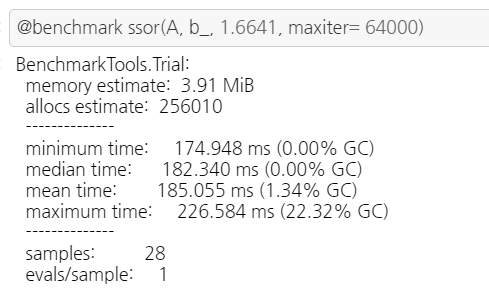
\includegraphics[width=0.4\textwidth]{benchmark_ssor_julia.png}%
        \label{fig:a}%
        }%
    \subfloat{%
        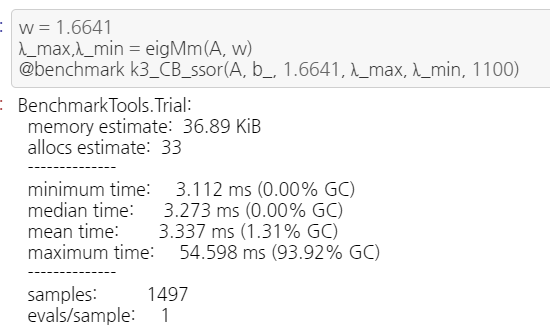
\includegraphics[width=0.4\textwidth]{benchmark_chebyssor_dw.png}%
        \label{fig:b}%
        }%
    \caption{Comparison between SSOR and Cheby-SSOR}
\end{figure}

Left shows the benchmark results of SSOR implemented in the Julia package
IterativeSolvers. Right shows the benchmark results of Cheby-SSOR implemented by us.
These shows that our implementation is much faster and memory efficient.
\end{frame}

\begin{frame}{Example 2. Biofilm image recovering}
    
\end{frame}


\end{document}